\documentclass[]{article}
\usepackage{lmodern}
\usepackage{amssymb,amsmath}
\usepackage{ifxetex,ifluatex}
\usepackage{fixltx2e} % provides \textsubscript
\ifnum 0\ifxetex 1\fi\ifluatex 1\fi=0 % if pdftex
  \usepackage[T1]{fontenc}
  \usepackage[utf8]{inputenc}
\else % if luatex or xelatex
  \ifxetex
    \usepackage{mathspec}
  \else
    \usepackage{fontspec}
  \fi
  \defaultfontfeatures{Ligatures=TeX,Scale=MatchLowercase}
\fi
% use upquote if available, for straight quotes in verbatim environments
\IfFileExists{upquote.sty}{\usepackage{upquote}}{}
% use microtype if available
\IfFileExists{microtype.sty}{%
\usepackage[]{microtype}
\UseMicrotypeSet[protrusion]{basicmath} % disable protrusion for tt fonts
}{}
\PassOptionsToPackage{hyphens}{url} % url is loaded by hyperref
\usepackage[unicode=true]{hyperref}
\hypersetup{
            pdftitle={Body Fat Data Analysis},
            pdfauthor={jdt},
            pdfborder={0 0 0},
            breaklinks=true}
\urlstyle{same}  % don't use monospace font for urls
\usepackage[margin=1in]{geometry}
\usepackage{color}
\usepackage{fancyvrb}
\newcommand{\VerbBar}{|}
\newcommand{\VERB}{\Verb[commandchars=\\\{\}]}
\DefineVerbatimEnvironment{Highlighting}{Verbatim}{commandchars=\\\{\}}
% Add ',fontsize=\small' for more characters per line
\usepackage{framed}
\definecolor{shadecolor}{RGB}{248,248,248}
\newenvironment{Shaded}{\begin{snugshade}}{\end{snugshade}}
\newcommand{\KeywordTok}[1]{\textcolor[rgb]{0.13,0.29,0.53}{\textbf{#1}}}
\newcommand{\DataTypeTok}[1]{\textcolor[rgb]{0.13,0.29,0.53}{#1}}
\newcommand{\DecValTok}[1]{\textcolor[rgb]{0.00,0.00,0.81}{#1}}
\newcommand{\BaseNTok}[1]{\textcolor[rgb]{0.00,0.00,0.81}{#1}}
\newcommand{\FloatTok}[1]{\textcolor[rgb]{0.00,0.00,0.81}{#1}}
\newcommand{\ConstantTok}[1]{\textcolor[rgb]{0.00,0.00,0.00}{#1}}
\newcommand{\CharTok}[1]{\textcolor[rgb]{0.31,0.60,0.02}{#1}}
\newcommand{\SpecialCharTok}[1]{\textcolor[rgb]{0.00,0.00,0.00}{#1}}
\newcommand{\StringTok}[1]{\textcolor[rgb]{0.31,0.60,0.02}{#1}}
\newcommand{\VerbatimStringTok}[1]{\textcolor[rgb]{0.31,0.60,0.02}{#1}}
\newcommand{\SpecialStringTok}[1]{\textcolor[rgb]{0.31,0.60,0.02}{#1}}
\newcommand{\ImportTok}[1]{#1}
\newcommand{\CommentTok}[1]{\textcolor[rgb]{0.56,0.35,0.01}{\textit{#1}}}
\newcommand{\DocumentationTok}[1]{\textcolor[rgb]{0.56,0.35,0.01}{\textbf{\textit{#1}}}}
\newcommand{\AnnotationTok}[1]{\textcolor[rgb]{0.56,0.35,0.01}{\textbf{\textit{#1}}}}
\newcommand{\CommentVarTok}[1]{\textcolor[rgb]{0.56,0.35,0.01}{\textbf{\textit{#1}}}}
\newcommand{\OtherTok}[1]{\textcolor[rgb]{0.56,0.35,0.01}{#1}}
\newcommand{\FunctionTok}[1]{\textcolor[rgb]{0.00,0.00,0.00}{#1}}
\newcommand{\VariableTok}[1]{\textcolor[rgb]{0.00,0.00,0.00}{#1}}
\newcommand{\ControlFlowTok}[1]{\textcolor[rgb]{0.13,0.29,0.53}{\textbf{#1}}}
\newcommand{\OperatorTok}[1]{\textcolor[rgb]{0.81,0.36,0.00}{\textbf{#1}}}
\newcommand{\BuiltInTok}[1]{#1}
\newcommand{\ExtensionTok}[1]{#1}
\newcommand{\PreprocessorTok}[1]{\textcolor[rgb]{0.56,0.35,0.01}{\textit{#1}}}
\newcommand{\AttributeTok}[1]{\textcolor[rgb]{0.77,0.63,0.00}{#1}}
\newcommand{\RegionMarkerTok}[1]{#1}
\newcommand{\InformationTok}[1]{\textcolor[rgb]{0.56,0.35,0.01}{\textbf{\textit{#1}}}}
\newcommand{\WarningTok}[1]{\textcolor[rgb]{0.56,0.35,0.01}{\textbf{\textit{#1}}}}
\newcommand{\AlertTok}[1]{\textcolor[rgb]{0.94,0.16,0.16}{#1}}
\newcommand{\ErrorTok}[1]{\textcolor[rgb]{0.64,0.00,0.00}{\textbf{#1}}}
\newcommand{\NormalTok}[1]{#1}
\usepackage{graphicx,grffile}
\makeatletter
\def\maxwidth{\ifdim\Gin@nat@width>\linewidth\linewidth\else\Gin@nat@width\fi}
\def\maxheight{\ifdim\Gin@nat@height>\textheight\textheight\else\Gin@nat@height\fi}
\makeatother
% Scale images if necessary, so that they will not overflow the page
% margins by default, and it is still possible to overwrite the defaults
% using explicit options in \includegraphics[width, height, ...]{}
\setkeys{Gin}{width=\maxwidth,height=\maxheight,keepaspectratio}
\IfFileExists{parskip.sty}{%
\usepackage{parskip}
}{% else
\setlength{\parindent}{0pt}
\setlength{\parskip}{6pt plus 2pt minus 1pt}
}
\setlength{\emergencystretch}{3em}  % prevent overfull lines
\providecommand{\tightlist}{%
  \setlength{\itemsep}{0pt}\setlength{\parskip}{0pt}}
\setcounter{secnumdepth}{0}
% Redefines (sub)paragraphs to behave more like sections
\ifx\paragraph\undefined\else
\let\oldparagraph\paragraph
\renewcommand{\paragraph}[1]{\oldparagraph{#1}\mbox{}}
\fi
\ifx\subparagraph\undefined\else
\let\oldsubparagraph\subparagraph
\renewcommand{\subparagraph}[1]{\oldsubparagraph{#1}\mbox{}}
\fi

% set default figure placement to htbp
\makeatletter
\def\fps@figure{htbp}
\makeatother


\title{Body Fat Data Analysis}
\author{jdt}
\date{11/10/2020}

\begin{document}
\maketitle

\begin{Shaded}
\begin{Highlighting}[]
  \CommentTok{# clear the environment and set seed}
\KeywordTok{rm}\NormalTok{(}\DataTypeTok{list =} \KeywordTok{ls}\NormalTok{())}
\KeywordTok{set.seed}\NormalTok{(}\DecValTok{123}\NormalTok{)}
\end{Highlighting}
\end{Shaded}

Read Body Fat Data

\begin{Shaded}
\begin{Highlighting}[]
\KeywordTok{library}\NormalTok{(foreign)}
\NormalTok{bfat =}\StringTok{ }\KeywordTok{read.dbf}\NormalTok{(}\StringTok{"new_bfat.dbf"}\NormalTok{)}
\end{Highlighting}
\end{Shaded}

Define a few variables

\begin{Shaded}
\begin{Highlighting}[]
\NormalTok{abdomen=bfat}\OperatorTok{$}\NormalTok{abdomen}
\NormalTok{thigh =}\StringTok{ }\NormalTok{bfat}\OperatorTok{$}\NormalTok{thigh}
\NormalTok{neck =}\StringTok{ }\NormalTok{bfat}\OperatorTok{$}\NormalTok{neck}
\NormalTok{per_fat =}\StringTok{ }\NormalTok{bfat}\OperatorTok{$}\NormalTok{per_fat}
\NormalTok{density =}\StringTok{ }\NormalTok{bfat}\OperatorTok{$}\NormalTok{density}
\NormalTok{age=bfat}\OperatorTok{$}\NormalTok{age}
\NormalTok{wt =}\StringTok{ }\NormalTok{bfat}\OperatorTok{$}\NormalTok{wt}
\NormalTok{ht =}\StringTok{ }\NormalTok{bfat}\OperatorTok{$}\NormalTok{ht}
\NormalTok{chest =}\StringTok{ }\NormalTok{bfat}\OperatorTok{$}\NormalTok{chest}
\NormalTok{hip =}\StringTok{ }\NormalTok{bfat}\OperatorTok{$}\NormalTok{hip}
\NormalTok{thigh =}\StringTok{ }\NormalTok{bfat}\OperatorTok{$}\NormalTok{thigh}
\NormalTok{knee =}\StringTok{ }\NormalTok{bfat}\OperatorTok{$}\NormalTok{knee}
\NormalTok{ankle =}\StringTok{ }\NormalTok{bfat}\OperatorTok{$}\NormalTok{ankle}
\NormalTok{biceps =}\StringTok{ }\NormalTok{bfat}\OperatorTok{$}\NormalTok{biceps}
\NormalTok{forearm =}\StringTok{ }\NormalTok{bfat}\OperatorTok{$}\NormalTok{forearm}
\NormalTok{wrist =}\StringTok{ }\NormalTok{bfat}\OperatorTok{$}\NormalTok{wrist}
\end{Highlighting}
\end{Shaded}

Plots of Percent Fat and Abdomen Circumference

\begin{Shaded}
\begin{Highlighting}[]
\KeywordTok{with}\NormalTok{(bfat, }\KeywordTok{hist}\NormalTok{(per_fat, }\DataTypeTok{main=}\StringTok{""}\NormalTok{, }\DataTypeTok{freq=}\OtherTok{FALSE}\NormalTok{))}
\KeywordTok{with}\NormalTok{(bfat, }\KeywordTok{lines}\NormalTok{(}\KeywordTok{density}\NormalTok{(per_fat), }\DataTypeTok{main=}\StringTok{"PERCENT FAT"}\NormalTok{, }\DataTypeTok{lty=}\DecValTok{2}\NormalTok{, }\DataTypeTok{lwd=}\DecValTok{2}\NormalTok{))}
\NormalTok{xvals =}\StringTok{ }\KeywordTok{with}\NormalTok{(bfat, }\KeywordTok{seq}\NormalTok{(}\DataTypeTok{from=}\KeywordTok{min}\NormalTok{(per_fat), }\DataTypeTok{to=}\KeywordTok{max}\NormalTok{(per_fat), }\DataTypeTok{length=}\DecValTok{100}\NormalTok{))}
\KeywordTok{with}\NormalTok{(bfat, }\KeywordTok{lines}\NormalTok{(xvals, }\KeywordTok{dnorm}\NormalTok{(xvals, }\KeywordTok{mean}\NormalTok{(per_fat), }\KeywordTok{sd}\NormalTok{(per_fat)), }\DataTypeTok{lwd=}\DecValTok{2}\NormalTok{))}
\end{Highlighting}
\end{Shaded}

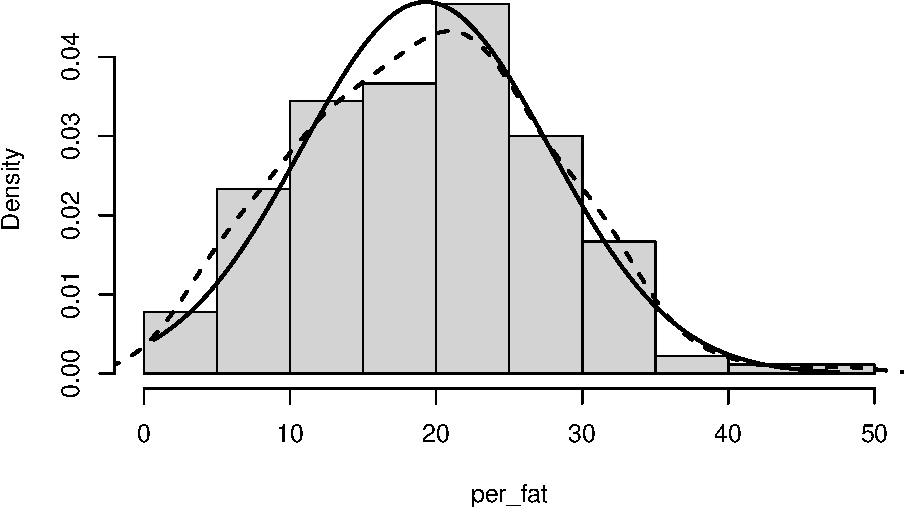
\includegraphics{BodyFat_files/figure-latex/unnamed-chunk-4-1.pdf}

\begin{Shaded}
\begin{Highlighting}[]
\KeywordTok{with}\NormalTok{(bfat, }\KeywordTok{hist}\NormalTok{(abdomen, }\DataTypeTok{main=}\StringTok{""}\NormalTok{, }\DataTypeTok{freq=}\OtherTok{FALSE}\NormalTok{))}
\KeywordTok{with}\NormalTok{(bfat, }\KeywordTok{lines}\NormalTok{(}\KeywordTok{density}\NormalTok{(abdomen), }\DataTypeTok{main=}\StringTok{"ABDOMEN"}\NormalTok{, }\DataTypeTok{lty=}\DecValTok{2}\NormalTok{, }\DataTypeTok{lwd=}\DecValTok{2}\NormalTok{))}
\NormalTok{xvals =}\StringTok{ }\KeywordTok{with}\NormalTok{(bfat, }\KeywordTok{seq}\NormalTok{(}\DataTypeTok{from=}\KeywordTok{min}\NormalTok{(abdomen), }\DataTypeTok{to=}\KeywordTok{max}\NormalTok{(abdomen), }\DataTypeTok{length=}\DecValTok{100}\NormalTok{))}
\KeywordTok{with}\NormalTok{(bfat, }\KeywordTok{lines}\NormalTok{(xvals, }\KeywordTok{dnorm}\NormalTok{(xvals, }\KeywordTok{mean}\NormalTok{(abdomen), }\KeywordTok{sd}\NormalTok{(abdomen)), }\DataTypeTok{lwd=}\DecValTok{2}\NormalTok{)) }
\end{Highlighting}
\end{Shaded}

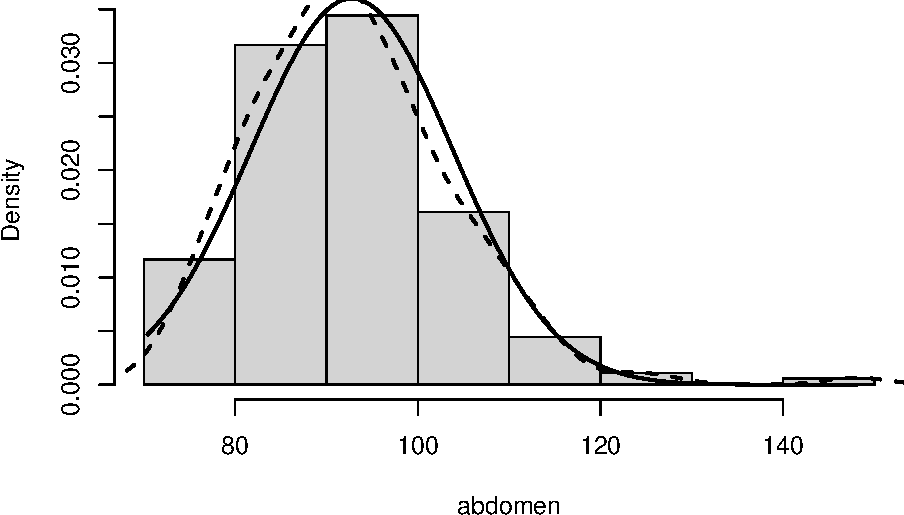
\includegraphics{BodyFat_files/figure-latex/unnamed-chunk-4-2.pdf}

Box Cox transformation for Abdomen

\begin{Shaded}
\begin{Highlighting}[]
\KeywordTok{library}\NormalTok{(MASS)}
\KeywordTok{boxcox}\NormalTok{(per_fat }\OperatorTok{~}\NormalTok{. ,}\DataTypeTok{data=}\NormalTok{bfat, }\DataTypeTok{lambda=}\KeywordTok{seq}\NormalTok{(}\OperatorTok{-}\NormalTok{.}\DecValTok{5}\NormalTok{, }\FloatTok{2.0}\NormalTok{, }\DataTypeTok{length=}\DecValTok{200}\NormalTok{))}
\end{Highlighting}
\end{Shaded}

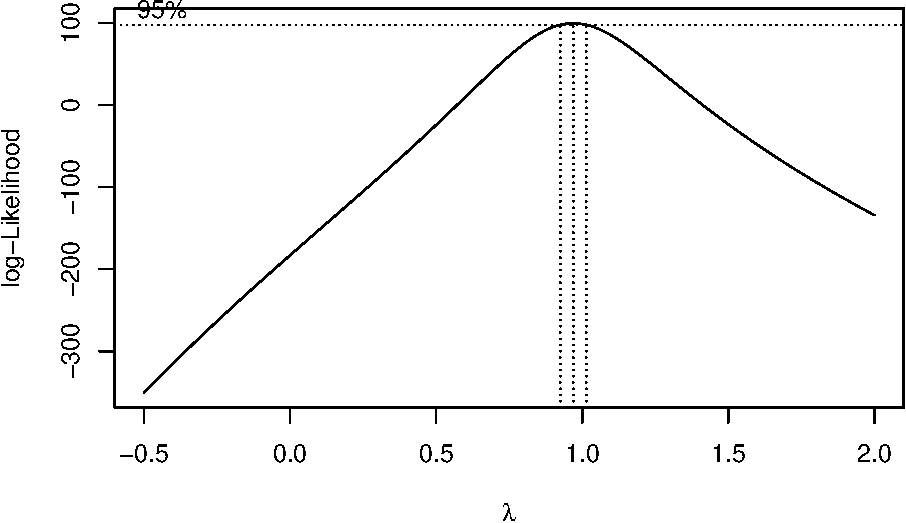
\includegraphics{BodyFat_files/figure-latex/unnamed-chunk-5-1.pdf}

\subsection{ROC Curves for High Percent
Fat}\label{roc-curves-for-high-percent-fat}

\begin{Shaded}
\begin{Highlighting}[]
\KeywordTok{library}\NormalTok{(ROCR)}
\CommentTok{#The code for the ROC with abdomen}
\NormalTok{disease=(per_fat }\OperatorTok{>}\StringTok{ }\DecValTok{26}\NormalTok{)}
\NormalTok{pred =}\StringTok{ }\KeywordTok{prediction}\NormalTok{(abdomen,disease)}
\NormalTok{perf=}\KeywordTok{performance}\NormalTok{(pred, }\StringTok{"tpr"}\NormalTok{, }\StringTok{"fpr"}\NormalTok{)}
\KeywordTok{plot}\NormalTok{(perf)}
\end{Highlighting}
\end{Shaded}

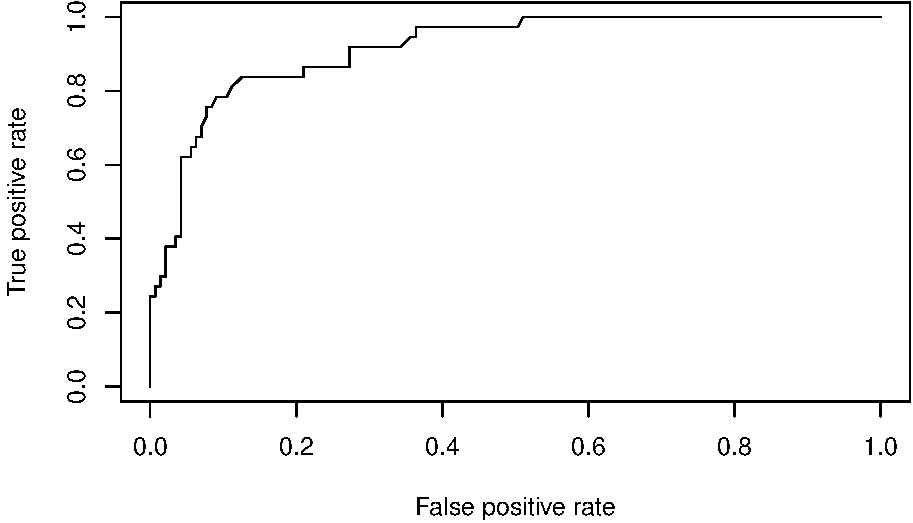
\includegraphics{BodyFat_files/figure-latex/unnamed-chunk-6-1.pdf}

\begin{Shaded}
\begin{Highlighting}[]
\CommentTok{# ROC for abdomen + thigh}
\NormalTok{pred =}\StringTok{ }\KeywordTok{prediction}\NormalTok{(abdomen }\OperatorTok{+}\StringTok{ }\NormalTok{thigh,disease) }
\NormalTok{perf=}\KeywordTok{performance}\NormalTok{(pred, }\StringTok{"tpr"}\NormalTok{, }\StringTok{"fpr"}\NormalTok{)}
\KeywordTok{plot}\NormalTok{(perf)}
\end{Highlighting}
\end{Shaded}

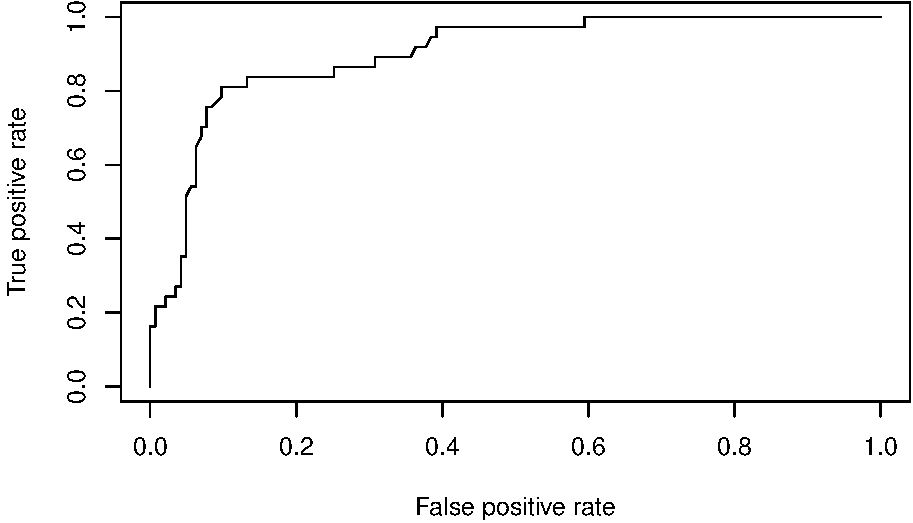
\includegraphics{BodyFat_files/figure-latex/unnamed-chunk-6-2.pdf}

\subsection{Linear Regression - model per\_fat =
abdomen}\label{linear-regression---model-per_fat-abdomen}

\begin{Shaded}
\begin{Highlighting}[]
\NormalTok{mod1 =}\StringTok{ }\KeywordTok{lm}\NormalTok{(per_fat }\OperatorTok{~}\StringTok{ }\NormalTok{abdomen, }\DataTypeTok{data=}\NormalTok{bfat)}
\KeywordTok{summary}\NormalTok{(mod1)}
\end{Highlighting}
\end{Shaded}

\begin{verbatim}
## 
## Call:
## lm(formula = per_fat ~ abdomen, data = bfat)
## 
## Residuals:
##      Min       1Q   Median       3Q      Max 
## -18.9840  -3.6341  -0.0102   3.4709  10.2028 
## 
## Coefficients:
##              Estimate Std. Error t value Pr(>|t|)    
## (Intercept) -39.22601    3.06172  -12.81   <2e-16 ***
## abdomen       0.63072    0.03277   19.25   <2e-16 ***
## ---
## Signif. codes:  0 '***' 0.001 '**' 0.01 '*' 0.05 '.' 0.1 ' ' 1
## 
## Residual standard error: 4.854 on 178 degrees of freedom
## Multiple R-squared:  0.6755, Adjusted R-squared:  0.6736 
## F-statistic: 370.5 on 1 and 178 DF,  p-value: < 2.2e-16
\end{verbatim}

\begin{Shaded}
\begin{Highlighting}[]
\NormalTok{covb =}\StringTok{ }\KeywordTok{vcov}\NormalTok{(mod1)}
\NormalTok{coeff.mod1 =}\StringTok{ }\KeywordTok{coef}\NormalTok{(mod1)}

\NormalTok{covb =}\StringTok{ }\KeywordTok{vcov}\NormalTok{(mod1)}
\NormalTok{covb}
\end{Highlighting}
\end{Shaded}

\begin{verbatim}
##             (Intercept)      abdomen
## (Intercept)  9.37412238 -0.099624319
## abdomen     -0.09962432  0.001073763
\end{verbatim}

\begin{Shaded}
\begin{Highlighting}[]
\NormalTok{pred.per_fat =}\StringTok{ }\KeywordTok{predict}\NormalTok{(mod1)}
\NormalTok{res.per_fat =}\StringTok{ }\KeywordTok{residuals}\NormalTok{(mod1)}
\KeywordTok{summary}\NormalTok{(res.per_fat)}
\end{Highlighting}
\end{Shaded}

\begin{verbatim}
##      Min.   1st Qu.    Median      Mean   3rd Qu.      Max. 
## -18.98400  -3.63414  -0.01023   0.00000   3.47087  10.20279
\end{verbatim}

Residual Plots

\begin{Shaded}
\begin{Highlighting}[]
\CommentTok{#par(mfrow=c(1,1))}
\KeywordTok{plot}\NormalTok{(mod1, }\DataTypeTok{which =} \KeywordTok{c}\NormalTok{(}\DecValTok{1}\NormalTok{, }\DecValTok{2}\NormalTok{))}
\end{Highlighting}
\end{Shaded}

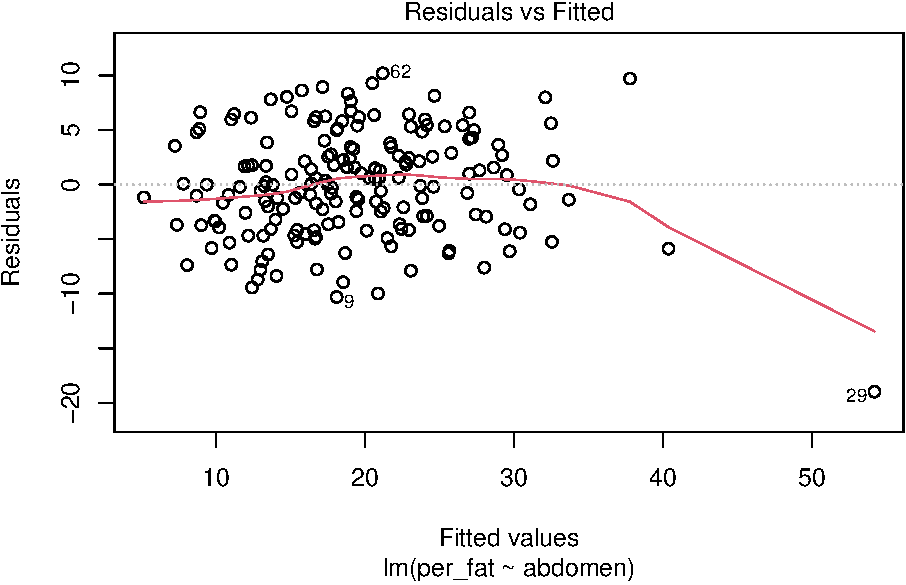
\includegraphics{BodyFat_files/figure-latex/unnamed-chunk-8-1.pdf}
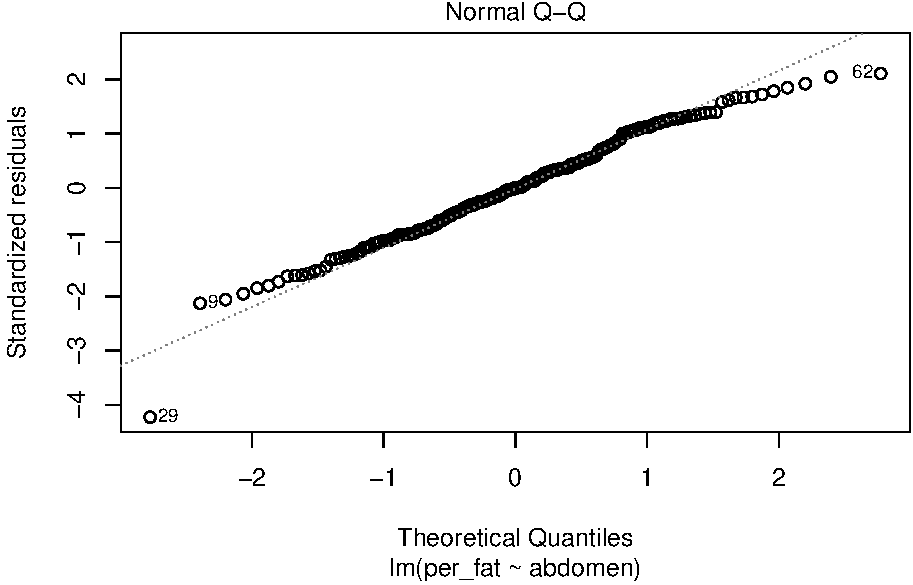
\includegraphics{BodyFat_files/figure-latex/unnamed-chunk-8-2.pdf}

\subsection{Multiple Regression}\label{multiple-regression}

\begin{Shaded}
\begin{Highlighting}[]
\NormalTok{mod2 =}\StringTok{ }\KeywordTok{lm}\NormalTok{(per_fat }\OperatorTok{~}\StringTok{ }\NormalTok{abdomen }\OperatorTok{+}\StringTok{ }\NormalTok{thigh }\OperatorTok{+}\StringTok{ }\NormalTok{neck, }\DataTypeTok{data=}\NormalTok{bfat)}
\KeywordTok{summary}\NormalTok{(mod2)}
\end{Highlighting}
\end{Shaded}

\begin{verbatim}
## 
## Call:
## lm(formula = per_fat ~ abdomen + thigh + neck, data = bfat)
## 
## Residuals:
##      Min       1Q   Median       3Q      Max 
## -14.9836  -3.4626   0.2172   3.1647   9.5368 
## 
## Coefficients:
##              Estimate Std. Error t value Pr(>|t|)    
## (Intercept) -15.92951    5.81094  -2.741  0.00675 ** 
## abdomen       0.83165    0.05705  14.578  < 2e-16 ***
## thigh        -0.08537    0.11205  -0.762  0.44712    
## neck         -0.96877    0.23741  -4.081  6.8e-05 ***
## ---
## Signif. codes:  0 '***' 0.001 '**' 0.01 '*' 0.05 '.' 0.1 ' ' 1
## 
## Residual standard error: 4.608 on 176 degrees of freedom
## Multiple R-squared:  0.7109, Adjusted R-squared:  0.7059 
## F-statistic: 144.2 on 3 and 176 DF,  p-value: < 2.2e-16
\end{verbatim}

Predicted values and Residuals

\begin{Shaded}
\begin{Highlighting}[]
\NormalTok{residual.per_fat=}\KeywordTok{residuals}\NormalTok{(mod2)}
\NormalTok{predicted.per_fat=}\KeywordTok{predict}\NormalTok{(mod2)}
\KeywordTok{plot}\NormalTok{(residual.per_fat, predicted.per_fat)}
\end{Highlighting}
\end{Shaded}

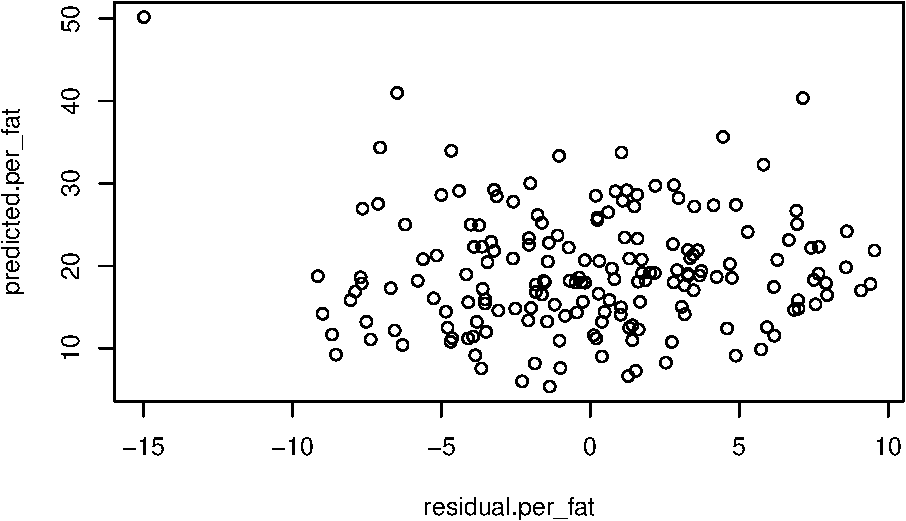
\includegraphics{BodyFat_files/figure-latex/unnamed-chunk-10-1.pdf}

\begin{Shaded}
\begin{Highlighting}[]
\KeywordTok{plot}\NormalTok{(per_fat, predicted.per_fat)}
\end{Highlighting}
\end{Shaded}

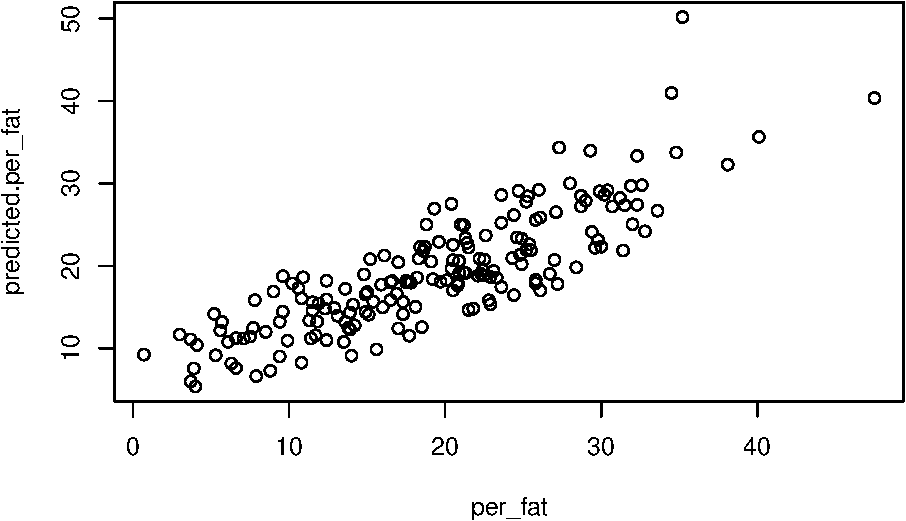
\includegraphics{BodyFat_files/figure-latex/unnamed-chunk-10-2.pdf}

\subsection{Model Selection}\label{model-selection}

\begin{Shaded}
\begin{Highlighting}[]
\CommentTok{#remove missing data}
\NormalTok{bfat =}\StringTok{ }\KeywordTok{na.omit}\NormalTok{(bfat)}
\NormalTok{colNames <-}\StringTok{ }\KeywordTok{colnames}\NormalTok{(bfat[,}\DecValTok{2}\OperatorTok{:}\DecValTok{14}\NormalTok{])}
\NormalTok{colNames}
\end{Highlighting}
\end{Shaded}

\begin{verbatim}
##  [1] "per_fat" "age"     "wt"      "ht"      "neck"    "chest"   "abdomen"
##  [8] "hip"     "thigh"   "knee"    "ankle"   "biceps"  "forearm"
\end{verbatim}

\begin{Shaded}
\begin{Highlighting}[]
\CommentTok{#Define a function to normalize data}

\NormalTok{normalize <-}\StringTok{ }\ControlFlowTok{function}\NormalTok{(df, cols) \{}
\NormalTok{  result <-}\StringTok{ }\NormalTok{df }\CommentTok{# make a copy of the input data frame}
    \ControlFlowTok{for}\NormalTok{ (j }\ControlFlowTok{in}\NormalTok{ cols) \{ }\CommentTok{# each specified col}
\NormalTok{    m <-}\StringTok{ }\KeywordTok{mean}\NormalTok{(df[,j]) }\CommentTok{# column mean}
\NormalTok{    std <-}\StringTok{ }\KeywordTok{sd}\NormalTok{(df[,j]) }\CommentTok{# column sd}

\NormalTok{    result[,j] <-}\StringTok{ }\KeywordTok{sapply}\NormalTok{(result[,j], }\ControlFlowTok{function}\NormalTok{(x) (x }\OperatorTok{-}\StringTok{ }\NormalTok{m) }\OperatorTok{/}\StringTok{ }\NormalTok{std)}
\NormalTok{    \}}
    \KeywordTok{return}\NormalTok{(result)}
\NormalTok{    \}}
    
\NormalTok{    bfat.norm <-}\StringTok{ }\KeywordTok{normalize}\NormalTok{(bfat, colNames)}
\NormalTok{    bfat.norm =}\StringTok{ }\NormalTok{bfat.norm[,}\DecValTok{2}\OperatorTok{:}\DecValTok{14}\NormalTok{]}
\end{Highlighting}
\end{Shaded}

Scatter Matrix for variables

\begin{Shaded}
\begin{Highlighting}[]
\KeywordTok{pairs}\NormalTok{(}\DataTypeTok{data=}\NormalTok{bfat, }\OperatorTok{~}\NormalTok{per_fat}\OperatorTok{+}\NormalTok{hip}\OperatorTok{+}\NormalTok{thigh}\OperatorTok{+}\NormalTok{knee}\OperatorTok{+}\NormalTok{ankle}\OperatorTok{+}\NormalTok{biceps}
      \OperatorTok{+}\NormalTok{forearm}\OperatorTok{+}\NormalTok{wrist)}
\end{Highlighting}
\end{Shaded}

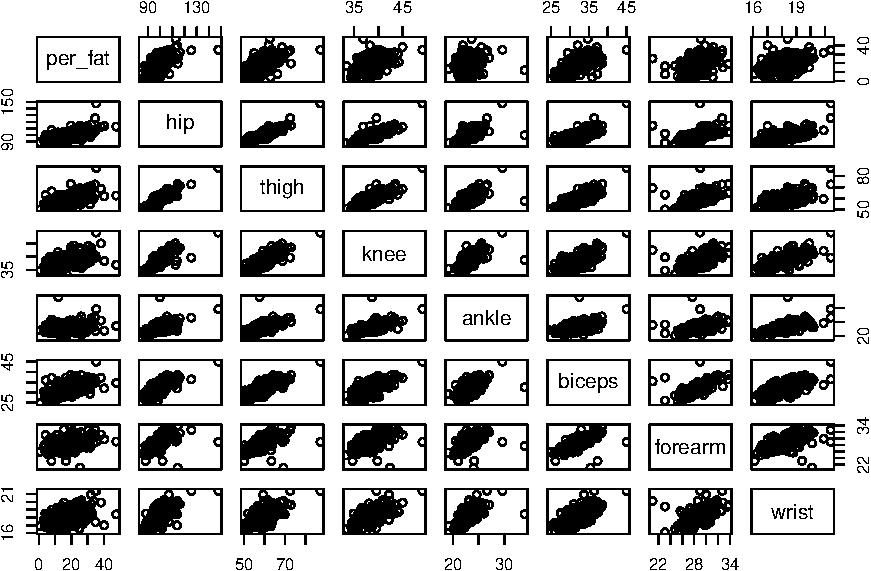
\includegraphics{BodyFat_files/figure-latex/unnamed-chunk-13-1.pdf}

\begin{Shaded}
\begin{Highlighting}[]
\NormalTok{model.null =}\StringTok{ }\KeywordTok{lm}\NormalTok{(per_fat }\OperatorTok{~}\StringTok{ }\DecValTok{1}\NormalTok{, }\DataTypeTok{data=}\NormalTok{bfat.norm)}
\NormalTok{model.full =}\StringTok{ }\KeywordTok{lm}\NormalTok{(per_fat }\OperatorTok{~}\NormalTok{., }\DataTypeTok{data=}\NormalTok{bfat.norm)}
\KeywordTok{summary.aov}\NormalTok{(model.null)}
\end{Highlighting}
\end{Shaded}

\begin{verbatim}
##              Df Sum Sq Mean Sq F value Pr(>F)
## Residuals   179    179       1
\end{verbatim}

\begin{Shaded}
\begin{Highlighting}[]
\KeywordTok{summary.aov}\NormalTok{(model.full)}
\end{Highlighting}
\end{Shaded}

\begin{verbatim}
##              Df Sum Sq Mean Sq F value   Pr(>F)    
## age           1  16.20   16.20  62.544 3.39e-13 ***
## wt            1  70.04   70.04 270.321  < 2e-16 ***
## ht            1  10.16   10.16  39.222 3.09e-09 ***
## neck          1   3.22    3.22  12.432 0.000545 ***
## chest         1   3.35    3.35  12.945 0.000422 ***
## abdomen       1  27.95   27.95 107.888  < 2e-16 ***
## hip           1   0.51    0.51   1.950 0.164490    
## thigh         1   2.58    2.58   9.971 0.001888 ** 
## knee          1   0.17    0.17   0.645 0.422930    
## ankle         1   0.18    0.18   0.710 0.400548    
## biceps        1   0.97    0.97   3.761 0.054135 .  
## forearm       1   0.38    0.38   1.485 0.224677    
## Residuals   167  43.27    0.26                     
## ---
## Signif. codes:  0 '***' 0.001 '**' 0.01 '*' 0.05 '.' 0.1 ' ' 1
\end{verbatim}

\subsection{Stepwise Model Selection}\label{stepwise-model-selection}

\begin{Shaded}
\begin{Highlighting}[]
\KeywordTok{step}\NormalTok{(model.null,}
     \DataTypeTok{scope =} \KeywordTok{list}\NormalTok{(}\DataTypeTok{upper=}\NormalTok{model.full),}
     \DataTypeTok{direction=}\StringTok{"both"}\NormalTok{, }\DataTypeTok{data=}\NormalTok{bfat.norm, }\DataTypeTok{trace =} \OtherTok{FALSE}\NormalTok{)  }
\end{Highlighting}
\end{Shaded}

\begin{verbatim}
## 
## Call:
## lm(formula = per_fat ~ abdomen + wt + biceps + neck, data = bfat.norm)
## 
## Coefficients:
## (Intercept)      abdomen           wt       biceps         neck  
##  -5.242e-16    1.295e+00   -5.233e-01    1.919e-01   -1.841e-01
\end{verbatim}

Final Model

\begin{Shaded}
\begin{Highlighting}[]
\NormalTok{model.final =}\StringTok{ }\KeywordTok{lm}\NormalTok{(}\DataTypeTok{formula =}\NormalTok{ per_fat }\OperatorTok{~}\StringTok{ }\NormalTok{abdomen }\OperatorTok{+}\StringTok{ }\NormalTok{hip }\OperatorTok{+}\StringTok{ }\NormalTok{wrist }
                 \OperatorTok{+}\StringTok{ }\NormalTok{thigh, }\DataTypeTok{data =}\NormalTok{ bfat.norm)}
\KeywordTok{summary}\NormalTok{(model.final)}
\end{Highlighting}
\end{Shaded}

\begin{verbatim}
## 
## Call:
## lm(formula = per_fat ~ abdomen + hip + wrist + thigh, data = bfat.norm)
## 
## Residuals:
##      Min       1Q   Median       3Q      Max 
## -1.42753 -0.34588 -0.05958  0.38643  1.21356 
## 
## Coefficients:
##             Estimate Std. Error t value Pr(>|t|)    
## (Intercept)  3.10953    1.00400   3.097  0.00228 ** 
## abdomen      1.21037    0.08222  14.720  < 2e-16 ***
## hip         -0.47987    0.11928  -4.023 8.54e-05 ***
## wrist       -0.17077    0.05510  -3.100  0.00226 ** 
## thigh        0.17253    0.09121   1.892  0.06019 .  
## ---
## Signif. codes:  0 '***' 0.001 '**' 0.01 '*' 0.05 '.' 0.1 ' ' 1
## 
## Residual standard error: 0.5254 on 175 degrees of freedom
## Multiple R-squared:  0.7301, Adjusted R-squared:  0.724 
## F-statistic: 118.4 on 4 and 175 DF,  p-value: < 2.2e-16
\end{verbatim}

\subsection{LASSO, Elastic Net and Ridge
Regression}\label{lasso-elastic-net-and-ridge-regression}

Stepwise regression assumes that the predictor variables are not highly
correlated. During each step in stepwise regression, a variable is
considered for addition to or subtraction from the set of predictor
variables based on some pre-specified criterion (e.g.~adjusted
R-squared). The two main approaches involve forward selection, starting
with no variables in the model, and backwards selection, starting with
all candidate predictors.

Lasso (least absolute shrinkage and selection operator) is a regression
analysis method that performs both variable selection and regularization
in order to enhance the prediction accuracy and interpretability of the
statistical model it produces.

The elastic net is a regularized regression method that linearly
combines the L1 and L2 penalties of the lasso and ridge methods. The
elastic net penalty is controlled by alpha, and bridges the gap between
lasso (alpha=1) and ridge (alpha=0). Note that the ridge penalty shrinks
the coefficients of correlated predictors towards each other while the
lasso tends to pick one and discard the others. Ridge is generally good
at prediction but tends to be less interpretable.

Data Preparation for Lasso and Ridge Regression

We will use the \texttt{glmnet} package in order to perform ridge
regression and lasso. The main function in this package is
\texttt{glmnet()}, which can be used to fit ridge regression models,
lasso models, and more. This function has a slightly different syntax
from other model-fitting functions that we have encountered thus far in
this book. In particular, we must pass in an \(x\) matrix as well as a
\(y\) vector, and we do not use the \(y \sim x\) syntax.

\begin{Shaded}
\begin{Highlighting}[]
\CommentTok{#Prepare Data for Lasso}
\CommentTok{#building lasso}

\NormalTok{XP=}\KeywordTok{data.matrix}\NormalTok{(bfat.norm[,}\OperatorTok{-}\DecValTok{1}\NormalTok{])}
\KeywordTok{summary}\NormalTok{(XP)}
\end{Highlighting}
\end{Shaded}

\begin{verbatim}
##       age                wt                 ht                neck         
##  Min.   :-1.8521   Min.   :-1.79051   Min.   :-2.39664   Min.   :-2.64721  
##  1st Qu.:-0.6386   1st Qu.:-0.64361   1st Qu.:-0.76438   1st Qu.:-0.66736  
##  Median :-0.1128   Median :-0.08466   Median :-0.04427   Median :-0.04108  
##  Mean   : 0.0000   Mean   : 0.00000   Mean   : 0.00000   Mean   : 0.00000  
##  3rd Qu.: 0.7366   3rd Qu.: 0.58609   3rd Qu.: 0.77185   3rd Qu.: 0.64581  
##  Max.   : 2.9208   Max.   : 6.09781   Max.   : 2.21208   Max.   : 5.31260  
##      chest            abdomen              hip               thigh         
##  Min.   :-2.0426   Min.   :-2.02119   Min.   :-1.98114   Min.   :-1.82517  
##  1st Qu.:-0.8146   1st Qu.:-0.75008   1st Qu.:-0.63176   1st Qu.:-0.64667  
##  Median :-0.1196   Median :-0.09759   Median :-0.07292   Median :-0.07674  
##  Mean   : 0.0000   Mean   : 0.00000   Mean   : 0.00000   Mean   : 0.00000  
##  3rd Qu.: 0.4857   3rd Qu.: 0.54362   3rd Qu.: 0.43480   3rd Qu.: 0.55115  
##  Max.   : 4.0740   Max.   : 4.99591   Max.   : 6.52405   Max.   : 5.38107  
##       knee              ankle             biceps            forearm        
##  Min.   :-2.19317   Min.   :-2.3968   Min.   :-2.51495   Min.   :-3.85106  
##  1st Qu.:-0.71889   1st Qu.:-0.6560   1st Qu.:-0.62450   1st Qu.:-0.66874  
##  Median :-0.08705   Median :-0.2358   Median :-0.07347   Median :-0.01207  
##  Mean   : 0.00000   Mean   : 0.0000   Mean   : 0.00000   Mean   : 0.00000  
##  3rd Qu.: 0.58691   3rd Qu.: 0.6046   3rd Qu.: 0.61320   3rd Qu.: 0.65723  
##  Max.   : 4.42004   Max.   : 6.4875   Max.   : 4.33475   Max.   : 2.61462
\end{verbatim}

\begin{Shaded}
\begin{Highlighting}[]
\NormalTok{x=XP}
\NormalTok{YP=}\KeywordTok{data.matrix}\NormalTok{(bfat.norm[,}\DecValTok{1}\NormalTok{])}
\KeywordTok{summary}\NormalTok{(YP)}
\end{Highlighting}
\end{Shaded}

\begin{verbatim}
##        V1         
##  Min.   :-2.1880  
##  1st Qu.:-0.7346  
##  Median : 0.0185  
##  Mean   : 0.0000  
##  3rd Qu.: 0.6952  
##  Max.   : 3.3194
\end{verbatim}

\begin{Shaded}
\begin{Highlighting}[]
\NormalTok{y=YP}
\NormalTok{lasso=}\KeywordTok{cv.glmnet}\NormalTok{(x, }
\NormalTok{                y, }\DataTypeTok{alpha=}\DecValTok{1}\NormalTok{,}
                \DataTypeTok{nfolds =} \DecValTok{5}\NormalTok{, }\DataTypeTok{type.measure=}\StringTok{"mse"}\NormalTok{, }
                \DataTypeTok{family=}\StringTok{"gaussian"}\NormalTok{)}
\end{Highlighting}
\end{Shaded}

Output the coefficients of the variables selected by lasso.

\begin{Shaded}
\begin{Highlighting}[]
\KeywordTok{coef}\NormalTok{(lasso, }\DataTypeTok{s=}\NormalTok{lasso}\OperatorTok{$}\NormalTok{lambda.min)}
\end{Highlighting}
\end{Shaded}

\begin{verbatim}
## 13 x 1 sparse Matrix of class "dgCMatrix"
##                         1
## (Intercept) -6.404803e-16
## age          6.885520e-02
## wt          -2.714618e-01
## ht           7.913540e-03
## neck        -2.146274e-01
## chest       -3.668275e-02
## abdomen      1.231445e+00
## hip         -2.277887e-01
## thigh        2.159657e-01
## knee        -3.105270e-02
## ankle       -5.329363e-02
## biceps       8.570149e-02
## forearm      6.167666e-02
\end{verbatim}

\subsection{Ridge Regression}\label{ridge-regression}

The \texttt{glmnet()} function has an alpha argument that determines
what type of model is fit. If \texttt{alpha\ =\ 0} then a ridge
regression model is fit, and if \texttt{alpha\ =\ 1} then a lasso model
is fit. We first fit a ridge regression model:

\begin{Shaded}
\begin{Highlighting}[]
\NormalTok{grid =}\StringTok{ }\DecValTok{10}\OperatorTok{^}\KeywordTok{seq}\NormalTok{(}\DecValTok{10}\NormalTok{, }\OperatorTok{-}\DecValTok{2}\NormalTok{, }\DataTypeTok{length =} \DecValTok{100}\NormalTok{)}
\NormalTok{ridge_mod =}\StringTok{ }\KeywordTok{glmnet}\NormalTok{(x, y, }\DataTypeTok{alpha =} \DecValTok{0}\NormalTok{, }\DataTypeTok{lambda =}\NormalTok{ grid)}
\end{Highlighting}
\end{Shaded}

By default the \texttt{glmnet()} function performs ridge regression for
an automatically selected range of \(\lambda\) values. However, here we
have chosen to implement the function over a grid of values ranging from
\(\lambda = 10^{10}\) to \(\lambda = 10^{-2}\), essentially covering the
full range of scenarios from the null model containing only the
intercept, to the least squares fit.

As we will see, we can also compute model fits for a particular value of
\(\lambda\) that is not one of the original grid values. Note that by
default, the \texttt{glmnet()} function standardizes the variables so
that they are on the same scale. To turn off this default setting use
the argument \texttt{standardize\ =\ FALSE}.

Associated with each value of \(\lambda\) is a vector of ridge
regression coefficients, stored in a matrix that can be accessed by
\texttt{coef()}. In this case, it is a \(15 \times 100\) matrix, with 15
rows (one for each predictor, plus an intercept) and 100 columns (one
for each value of \(\lambda\)).

\begin{Shaded}
\begin{Highlighting}[]
\KeywordTok{dim}\NormalTok{(}\KeywordTok{coef}\NormalTok{(ridge_mod))}
\end{Highlighting}
\end{Shaded}

\begin{verbatim}
## [1]  13 100
\end{verbatim}

\begin{Shaded}
\begin{Highlighting}[]
\KeywordTok{plot}\NormalTok{(ridge_mod)    }\CommentTok{# Draw plot of coefficients}
\end{Highlighting}
\end{Shaded}

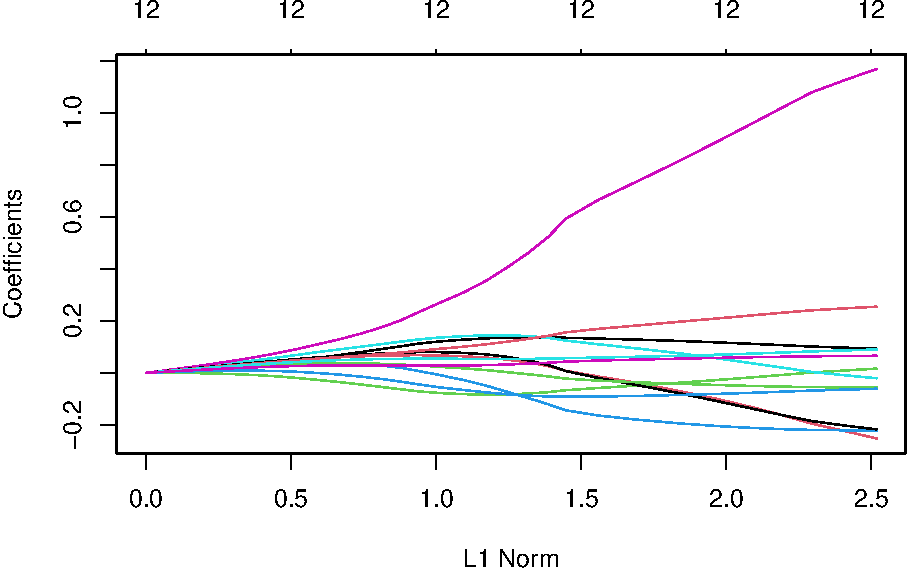
\includegraphics{BodyFat_files/figure-latex/unnamed-chunk-22-1.pdf}

We expect the coefficient estimates to be much smaller, in terms of
\(l_2\) norm when a large value of \(\lambda\) is used, as compared to
when a small value of \(\lambda\) is used. These are the coefficients
when \(\lambda = 11498\), along with their \(l_2\) norm:

\begin{Shaded}
\begin{Highlighting}[]
\NormalTok{ridge_mod}\OperatorTok{$}\NormalTok{lambda[}\DecValTok{50}\NormalTok{] }\CommentTok{# Display 50th lambda value"}
\end{Highlighting}
\end{Shaded}

\begin{verbatim}
## [1] 11497.57
\end{verbatim}

\begin{Shaded}
\begin{Highlighting}[]
\KeywordTok{coef}\NormalTok{(ridge_mod)[,}\DecValTok{50}\NormalTok{] }\CommentTok{# Display coefficients associated with 50th lambda value"}
\end{Highlighting}
\end{Shaded}

\begin{verbatim}
##   (Intercept)           age            wt            ht          neck 
## -1.526432e-16  2.609254e-05  5.445809e-05  1.388594e-06  4.591450e-05 
##         chest       abdomen           hip         thigh          knee 
##  6.161509e-05  7.125235e-05  5.440005e-05  5.053996e-05  4.333254e-05 
##         ankle        biceps       forearm 
##  2.307746e-05  4.685840e-05  3.369981e-05
\end{verbatim}

\begin{Shaded}
\begin{Highlighting}[]
\KeywordTok{sqrt}\NormalTok{(}\KeywordTok{sum}\NormalTok{(}\KeywordTok{coef}\NormalTok{(ridge_mod)[}\OperatorTok{-}\DecValTok{1}\NormalTok{,}\DecValTok{50}\NormalTok{]}\OperatorTok{^}\DecValTok{2}\NormalTok{)) }\CommentTok{# Calculate l2 norm"}
\end{Highlighting}
\end{Shaded}

\begin{verbatim}
## [1] 0.0001608888
\end{verbatim}

In contrast, here are the coefficients when \(\lambda = 705\), along
with their \(l_2\) norm. Note the much larger \(l_2\) norm of the
coefficients associated with this smaller value of \(\lambda\)."

\begin{Shaded}
\begin{Highlighting}[]
\NormalTok{ridge_mod}\OperatorTok{$}\NormalTok{lambda[}\DecValTok{60}\NormalTok{] }\CommentTok{#Display 60th lambda value\textbackslash{}n",}
\end{Highlighting}
\end{Shaded}

\begin{verbatim}
## [1] 705.4802
\end{verbatim}

\begin{Shaded}
\begin{Highlighting}[]
\KeywordTok{coef}\NormalTok{(ridge_mod)[,}\DecValTok{60}\NormalTok{] }\CommentTok{# Display coefficients associated with 60th lambda value\textbackslash{}n",}
\end{Highlighting}
\end{Shaded}

\begin{verbatim}
##   (Intercept)           age            wt            ht          neck 
## -1.524550e-16  4.243217e-04  8.804158e-04  2.003903e-05  7.415898e-04 
##         chest       abdomen           hip         thigh          knee 
##  9.969227e-04  1.153624e-03  8.787311e-04  8.159913e-04  6.985972e-04 
##         ankle        biceps       forearm 
##  3.701699e-04  7.558705e-04  5.429845e-04
\end{verbatim}

\begin{Shaded}
\begin{Highlighting}[]
\KeywordTok{sqrt}\NormalTok{(}\KeywordTok{sum}\NormalTok{(}\KeywordTok{coef}\NormalTok{(ridge_mod)[}\OperatorTok{-}\DecValTok{1}\NormalTok{,}\DecValTok{60}\NormalTok{]}\OperatorTok{^}\DecValTok{2}\NormalTok{)) }\CommentTok{# Calculate l2 norm"}
\end{Highlighting}
\end{Shaded}

\begin{verbatim}
## [1] 0.002599901
\end{verbatim}

We can use the \texttt{predict()} function for a number of purposes. For
instance we can obtain the ridge regression coefficients for a new value
of \(\lambda\), say 50:

\begin{Shaded}
\begin{Highlighting}[]
\KeywordTok{predict}\NormalTok{(ridge_mod, }\DataTypeTok{s =} \DecValTok{50}\NormalTok{, }\DataTypeTok{type =}  \StringTok{"coefficients"}\NormalTok{)}
\end{Highlighting}
\end{Shaded}

\begin{verbatim}
## 13 x 1 sparse Matrix of class "dgCMatrix"
##                         1
## (Intercept) -1.503188e-16
## age          5.895880e-03
## wt           1.101510e-02
## ht          -2.948972e-04
## neck         9.170962e-03
## chest        1.278125e-02
## abdomen      1.503427e-02
## hip          1.107665e-02
## thigh        1.025128e-02
## knee         8.615043e-03
## ankle        4.224826e-03
## biceps       9.446253e-03
## forearm      6.691531e-03
\end{verbatim}

We now split the samples into a training set and a test set in order to
estimate the test error of ridge regression and the lasso.

\begin{Shaded}
\begin{Highlighting}[]
\KeywordTok{set.seed}\NormalTok{(}\DecValTok{1}\NormalTok{)}
    
\NormalTok{train =}\StringTok{ }\NormalTok{bfat.norm }\OperatorTok
\StringTok{  }\KeywordTok{sample_frac}\NormalTok{(}\FloatTok{0.5}\NormalTok{)}
    
\NormalTok{test =}\StringTok{ }\NormalTok{bfat.norm }\OperatorTok
\StringTok{  }\KeywordTok{setdiff}\NormalTok{(train)}

\NormalTok{d_train =}\StringTok{ }\NormalTok{train[,}\OperatorTok{-}\DecValTok{1}\NormalTok{]}
\NormalTok{d_test =}\StringTok{ }\NormalTok{test[,}\OperatorTok{-}\DecValTok{1}\NormalTok{]}
\NormalTok{x_train =}\StringTok{ }\KeywordTok{model.matrix}\NormalTok{(train}\OperatorTok{$}\NormalTok{per_fat}\OperatorTok{~}\NormalTok{., }\DataTypeTok{data=}\NormalTok{d_train)}
\NormalTok{x_test =}\StringTok{ }\KeywordTok{model.matrix}\NormalTok{(test}\OperatorTok{$}\NormalTok{per_fat}\OperatorTok{~}\NormalTok{., }\DataTypeTok{data=}\NormalTok{d_test)}
  
\NormalTok{y_train =}\StringTok{ }\NormalTok{train }\OperatorTok
\StringTok{  }\KeywordTok{select}\NormalTok{(per_fat) }\OperatorTok
\StringTok{  }\KeywordTok{unlist}\NormalTok{() }\OperatorTok
\StringTok{  }\KeywordTok{as.numeric}\NormalTok{()}

\NormalTok{y_test =}\StringTok{ }\NormalTok{test }\OperatorTok
\StringTok{  }\KeywordTok{select}\NormalTok{(per_fat) }\OperatorTok
\StringTok{  }\KeywordTok{unlist}\NormalTok{() }\OperatorTok
\StringTok{  }\KeywordTok{as.numeric}\NormalTok{()}
\end{Highlighting}
\end{Shaded}

Next we fit a ridge regression model on the training set, and evaluate
its MSE on the test set, using \(\lambda = 4\). Note the use of the
\texttt{predict()} function again: this time we get predictions for a
test set, by replacing
\texttt{type=\textbackslash{}"coefficients\textbackslash{}"} with the
\texttt{newx} argument.

\begin{Shaded}
\begin{Highlighting}[]
\NormalTok{ridge_mod =}\StringTok{ }\KeywordTok{glmnet}\NormalTok{(x_train, y_train, }\DataTypeTok{alpha=}\DecValTok{0}\NormalTok{, }\DataTypeTok{lambda =}\NormalTok{ grid, }\DataTypeTok{thresh =} \FloatTok{1e-12}\NormalTok{)}
\NormalTok{ridge_pred =}\StringTok{ }\KeywordTok{predict}\NormalTok{(ridge_mod, }\DataTypeTok{s =} \DecValTok{4}\NormalTok{, }\DataTypeTok{newx =}\NormalTok{ x_test)}
\KeywordTok{mean}\NormalTok{((ridge_pred }\OperatorTok{-}\StringTok{ }\NormalTok{y_test)}\OperatorTok{^}\DecValTok{2}\NormalTok{)}
\end{Highlighting}
\end{Shaded}

\begin{verbatim}
## [1] 0.6560573
\end{verbatim}

The test MSE is 101242.7. Note that if we had instead simply fit a model
with just an intercept, we would have predicted each test observation
using the mean of the training observations. In that case, we could
compute the test set MSE like this:

\begin{Shaded}
\begin{Highlighting}[]
\KeywordTok{mean}\NormalTok{((}\KeywordTok{mean}\NormalTok{(y_train) }\OperatorTok{-}\StringTok{ }\NormalTok{y_test)}\OperatorTok{^}\DecValTok{2}\NormalTok{)}
\end{Highlighting}
\end{Shaded}

\begin{verbatim}
## [1] 1.071273
\end{verbatim}

We could also get the same result by fitting a ridge regression model
with a very large value of \(\lambda\). Note that \texttt{1e10} means
\(10^{10}\).

\begin{Shaded}
\begin{Highlighting}[]
\NormalTok{ridge_pred =}\StringTok{ }\KeywordTok{predict}\NormalTok{(ridge_mod, }\DataTypeTok{s =} \FloatTok{1e10}\NormalTok{, }\DataTypeTok{newx =}\NormalTok{ x_test)}
\KeywordTok{mean}\NormalTok{((ridge_pred }\OperatorTok{-}\StringTok{ }\NormalTok{y_test)}\OperatorTok{^}\DecValTok{2}\NormalTok{)}
\end{Highlighting}
\end{Shaded}

\begin{verbatim}
## [1] 1.071273
\end{verbatim}

So fitting a ridge regression model with \(\lambda = 4\) leads to a much
lower test MSE than fitting a model with just an intercept. We now check
whether there is any benefit to performing ridge regression with
\(\lambda = 4\) instead of just performing least squares regression.
Recall that least squares is simply ridge regression with
\(\lambda = 0\).

* Note: In order for \texttt{glmnet()} to yield the \textbf{exact} least
squares coefficients when \(\lambda = 0\) we use the argument
\texttt{exact=T} when calling the \texttt{predict()} function.
Otherwise, the \texttt{predict()} function will interpolate over the
grid of \(\lambda\) values used in fitting the \texttt{glmnet()} model,
yielding approximate results. Even when we use \texttt{exact\ =\ TRUE},
there remains a slight discrepancy in the third decimal place between
the output of \texttt{glmnet()} when \(\lambda = 0\) and the output of
\texttt{lm()}; this is due to numerical approximation on the part of
\texttt{glmnet()}.

\begin{Shaded}
\begin{Highlighting}[]
\NormalTok{ridge_pred =}\StringTok{ }\KeywordTok{predict}\NormalTok{(ridge_mod, }\DataTypeTok{s =} \DecValTok{0}\NormalTok{, }\DataTypeTok{newx =}\NormalTok{ x_test, }\DataTypeTok{exact =} \OtherTok{FALSE}\NormalTok{)}
\KeywordTok{mean}\NormalTok{((ridge_pred }\OperatorTok{-}\StringTok{ }\NormalTok{y_test)}\OperatorTok{^}\DecValTok{2}\NormalTok{)}
\end{Highlighting}
\end{Shaded}

\begin{verbatim}
## [1] 0.2939128
\end{verbatim}

\begin{Shaded}
\begin{Highlighting}[]
\KeywordTok{lm}\NormalTok{(per_fat}\OperatorTok{~}\NormalTok{., }\DataTypeTok{data =}\NormalTok{ train)}
\end{Highlighting}
\end{Shaded}

\begin{verbatim}
## 
## Call:
## lm(formula = per_fat ~ ., data = train)
## 
## Coefficients:
## (Intercept)          age           wt           ht         neck        chest  
##    -0.04207      0.06705     -0.10845      0.06784     -0.11087     -0.11178  
##     abdomen          hip        thigh         knee        ankle       biceps  
##     1.20913     -0.36838      0.30119     -0.17599     -0.06556      0.01185  
##     forearm  
##     0.11493
\end{verbatim}

\begin{Shaded}
\begin{Highlighting}[]
\KeywordTok{predict}\NormalTok{(ridge_mod, }\DataTypeTok{s =} \DecValTok{0}\NormalTok{, }\DataTypeTok{exact =} \OtherTok{FALSE}\NormalTok{, }\DataTypeTok{type=}\StringTok{"coefficients"}\NormalTok{)}
\end{Highlighting}
\end{Shaded}

\begin{verbatim}
## 14 x 1 sparse Matrix of class "dgCMatrix"
##                       1
## (Intercept) -0.03975030
## (Intercept)  .         
## age          0.08942505
## wt          -0.09216846
## ht           0.06019398
## neck        -0.11133160
## chest       -0.03786918
## abdomen      1.04018522
## hip         -0.26435594
## thigh        0.27130829
## knee        -0.17971659
## ankle       -0.07036256
## biceps       0.02012120
## forearm      0.10807213
\end{verbatim}

It looks like we are indeed improving over regular least-squares! Side
note: in general, if we want to fit a (unpenalized) least squares model,
then we should use the \texttt{lm()} function, since that function
provides more useful outputs, such as standard errors and \(p\)-values
for the coefficients.

Instead of arbitrarily choosing \(\lambda = 4\), it would be better to
use cross-validation to choose the tuning parameter \(\lambda\). We can
do this using the built-in cross-validation function,
\texttt{cv.glmnet()}. By default, the function performs 10-fold
cross-validation, though this can be changed using the argument
\texttt{folds}. Note that we set a random seed first so our results will
be reproducible, since the choice of the cross-validation folds is
random.

\begin{Shaded}
\begin{Highlighting}[]
\KeywordTok{set.seed}\NormalTok{(}\DecValTok{1}\NormalTok{)}

\NormalTok{cv.out =}\StringTok{ }\KeywordTok{cv.glmnet}\NormalTok{(x_train, y_train, }\DataTypeTok{alpha =} \DecValTok{0}\NormalTok{) }\CommentTok{# Fit ridge regression model on training data}
\NormalTok{bestlam =}\StringTok{ }\NormalTok{cv.out}\OperatorTok{$}\NormalTok{lambda.min  }\CommentTok{# Select lamda that minimizes training MSE}
\NormalTok{bestlam}
\end{Highlighting}
\end{Shaded}

\begin{verbatim}
## [1] 0.07850514
\end{verbatim}

Therefore, we see that the value of \(\lambda\) that results in the
smallest cross-validation error is 339.1845 We can also plot the MSE as
a function of \(\lambda\):

\begin{Shaded}
\begin{Highlighting}[]
\KeywordTok{plot}\NormalTok{(cv.out) }\CommentTok{# Draw plot of training MSE as a function of lambda}
\end{Highlighting}
\end{Shaded}

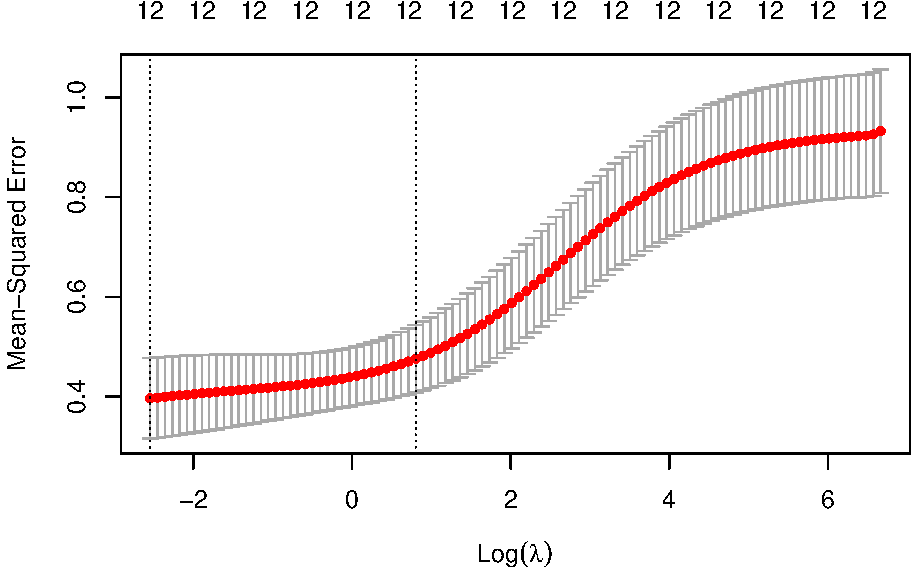
\includegraphics{BodyFat_files/figure-latex/unnamed-chunk-34-1.pdf}

What is the test MSE associated with this value of \(\lambda\)?

\begin{Shaded}
\begin{Highlighting}[]
\NormalTok{ridge_pred =}\StringTok{ }\KeywordTok{predict}\NormalTok{(ridge_mod, }\DataTypeTok{s =}\NormalTok{ bestlam, }\DataTypeTok{newx =}\NormalTok{ x_test) }\CommentTok{# Use best lambda to predict test data}
\KeywordTok{mean}\NormalTok{((ridge_pred }\OperatorTok{-}\StringTok{ }\NormalTok{y_test)}\OperatorTok{^}\DecValTok{2}\NormalTok{) }\CommentTok{# Calculate test MSE}
\end{Highlighting}
\end{Shaded}

\begin{verbatim}
## [1] 0.3473058
\end{verbatim}

This represents a further improvement over the test MSE that we got
using \(\lambda = 4\). Finally, we refit our ridge regression model on
the full data set using the value of \(\lambda\) chosen by
cross-validation, and examine the coefficient estimates.

\begin{Shaded}
\begin{Highlighting}[]
\NormalTok{out =}\StringTok{ }\KeywordTok{glmnet}\NormalTok{(x, y, }\DataTypeTok{alpha =} \DecValTok{0}\NormalTok{) }\CommentTok{# Fit ridge regression model on full dataset}
\KeywordTok{predict}\NormalTok{(out, }\DataTypeTok{type =} \StringTok{"coefficients"}\NormalTok{, }\DataTypeTok{s =}\NormalTok{ bestlam) }\CommentTok{# Display coefficients using lambda chosen by CV}
\end{Highlighting}
\end{Shaded}

\begin{verbatim}
## 13 x 1 sparse Matrix of class "dgCMatrix"
##                         1
## (Intercept) -5.369552e-16
## age          1.298104e-01
## wt          -2.686305e-02
## ht          -5.341804e-02
## neck        -1.722698e-01
## chest        1.033859e-01
## abdomen      7.002786e-01
## hip         -3.260382e-02
## thigh        1.759446e-01
## knee        -3.318926e-02
## ankle       -9.015065e-02
## biceps       5.988103e-02
## forearm      4.888949e-02
\end{verbatim}

As expected, none of the coefficients are exactly zero - ridge
regression does not perform variable selection!

\subsection{The Lasso}\label{the-lasso}

We saw that ridge regression with a wise choice of \(\lambda\) can
outperform least squares as well as the null model on the Hitters data
set. We now ask whether the lasso can yield either a more accurate or a
more interpretable model than ridge regression. In order to fit a lasso
model, we once again use the \texttt{glmnet()} function; however, this
time we use the argument \texttt{alpha=1}. Other than that change, we
proceed just as we did in fitting a ridge model:

\begin{Shaded}
\begin{Highlighting}[]
\NormalTok{lasso_mod =}\StringTok{ }\KeywordTok{glmnet}\NormalTok{(x_train, }
\NormalTok{                   y_train, }
                   \DataTypeTok{alpha =} \DecValTok{1}\NormalTok{, }
                   \DataTypeTok{lambda =}\NormalTok{ grid) }\CommentTok{# Fit lasso model on training data}

\KeywordTok{plot}\NormalTok{(lasso_mod)    }\CommentTok{# Draw plot of coefficients}
\end{Highlighting}
\end{Shaded}

\begin{verbatim}
## Warning in regularize.values(x, y, ties, missing(ties), na.rm = na.rm):
## collapsing to unique 'x' values
\end{verbatim}

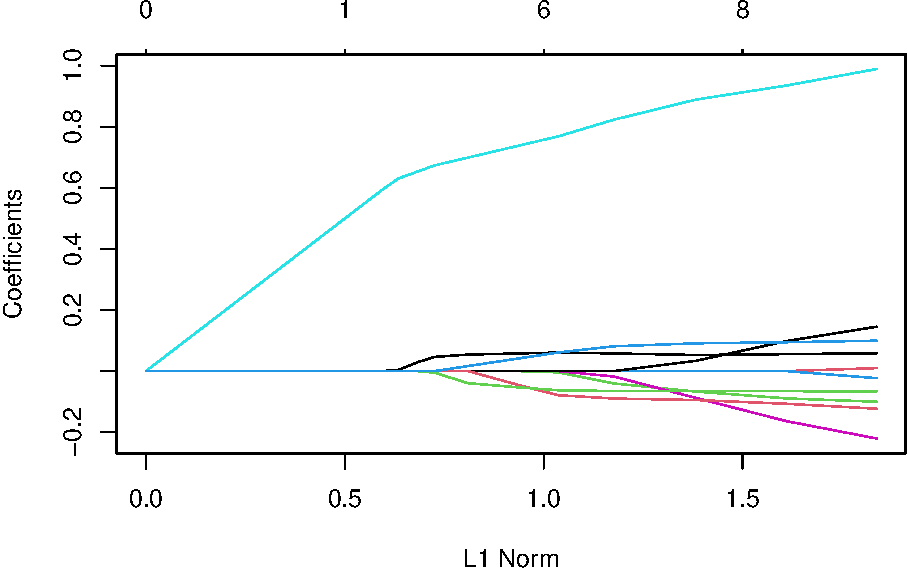
\includegraphics{BodyFat_files/figure-latex/unnamed-chunk-37-1.pdf}

Notice that in the coefficient plot that depending on the choice of
tuning parameter, some of the coefficients are exactly equal to zero. We
now perform cross-validation and compute the associated test error:

\begin{Shaded}
\begin{Highlighting}[]
\KeywordTok{set.seed}\NormalTok{(}\DecValTok{1}\NormalTok{)}
\NormalTok{cv.out =}\StringTok{ }\KeywordTok{cv.glmnet}\NormalTok{(x_train, y_train, }\DataTypeTok{alpha =} \DecValTok{1}\NormalTok{) }\CommentTok{# Fit lasso model on training data}
\KeywordTok{plot}\NormalTok{(cv.out) }\CommentTok{# Draw plot of training MSE as a function of lambda}
\end{Highlighting}
\end{Shaded}

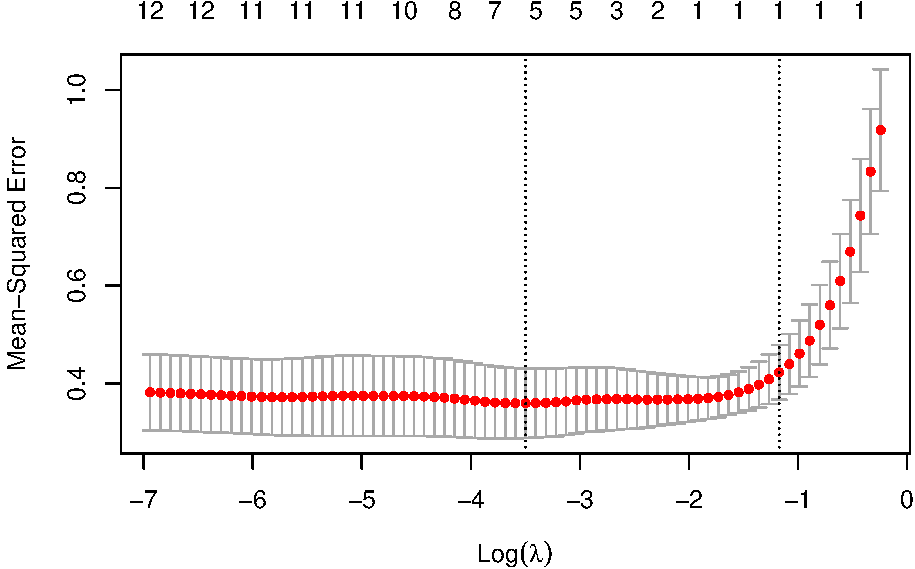
\includegraphics{BodyFat_files/figure-latex/unnamed-chunk-38-1.pdf}

\begin{Shaded}
\begin{Highlighting}[]
\NormalTok{bestlam =}\StringTok{ }\NormalTok{cv.out}\OperatorTok{$}\NormalTok{lambda.min }\CommentTok{# Select lamda that minimizes training MSE}
\NormalTok{lasso_pred =}\StringTok{ }\KeywordTok{predict}\NormalTok{(lasso_mod, }\DataTypeTok{s =}\NormalTok{ bestlam, }\DataTypeTok{newx =}\NormalTok{ x_test) }\CommentTok{# Use best lambda to predict test data}
\KeywordTok{mean}\NormalTok{((lasso_pred }\OperatorTok{-}\StringTok{ }\NormalTok{y_test)}\OperatorTok{^}\DecValTok{2}\NormalTok{) }\CommentTok{# Calculate test MSE}
\end{Highlighting}
\end{Shaded}

\begin{verbatim}
## [1] 0.3392375
\end{verbatim}

This is substantially lower than the test set MSE of the null model and
of least squares, and very similar to the test MSE of ridge regression
with \(\lambda\) chosen by cross-validation.

However, the lasso has a substantial advantage over ridge regression in
that the resulting coefficient estimates are sparse. Here we see that 12
of the 14 coefficient estimates are exactly zero:

\begin{Shaded}
\begin{Highlighting}[]
\NormalTok{out =}\StringTok{ }\KeywordTok{glmnet}\NormalTok{(x, y, }\DataTypeTok{alpha =} \DecValTok{1}\NormalTok{, }\DataTypeTok{lambda =}\NormalTok{ grid) }\CommentTok{# Fit lasso model on full dataset}
\NormalTok{lasso_coef =}\StringTok{ }\KeywordTok{predict}\NormalTok{(out, }\DataTypeTok{type =} \StringTok{"coefficients"}\NormalTok{, }
\DataTypeTok{s =}\NormalTok{ bestlam) }\CommentTok{# Display coefficients using lambda chosen by CV}
\NormalTok{lasso_coef}
\end{Highlighting}
\end{Shaded}

\begin{verbatim}
## 13 x 1 sparse Matrix of class "dgCMatrix"
##                         1
## (Intercept) -5.488650e-16
## age          5.148006e-02
## wt           .           
## ht          -4.491412e-02
## neck        -1.127499e-01
## chest        .           
## abdomen      8.975255e-01
## hip         -6.285664e-04
## thigh        .           
## knee         .           
## ankle       -6.341860e-02
## biceps       3.817580e-04
## forearm      1.963505e-02
\end{verbatim}

Selecting only the predictors with non-zero (greater than 1e-02)
coefficients, we see that the lasso model with \(\lambda\) chosen by
cross-validation contains only seven variables:

\begin{Shaded}
\begin{Highlighting}[]
\NormalTok{lasso_coef[lasso_coef }\OperatorTok{>}\StringTok{ }\FloatTok{1e-02}\NormalTok{] }\CommentTok{# Display only non-zero coefficients}
\end{Highlighting}
\end{Shaded}

\begin{verbatim}
## <sparse>[ <logic> ] : .M.sub.i.logical() maybe inefficient
\end{verbatim}

\begin{verbatim}
## [1] 0.05148006 0.89752545 0.01963505
\end{verbatim}

\subsection{Check for
Multcollinearity}\label{check-for-multcollinearity}

This file produces the resulte for VIF using R

\subsection{Method 1}\label{method-1}

\begin{verbatim}
##    Variables       VIF
## 1    per_fat  4.136974
## 2        age  1.877750
## 3         wt 47.879102
## 4         ht  3.017498
## 5       neck  4.871078
## 6      chest 11.262578
## 7    abdomen 19.457248
## 8        hip 15.475037
## 9      thigh  9.126259
## 10      knee  5.010651
## 11     ankle  2.207485
## 12    biceps  4.343836
## 13   forearm  2.170823
\end{verbatim}

\subsection{Method 2}\label{method-2}

\begin{Shaded}
\begin{Highlighting}[]
\CommentTok{# Source of function is }
\CommentTok{# http://highstat.com/Books/BGS/GAMM/RCodeP2/HighstatLibV6.R}

\CommentTok{#To use:  corvif(YourDataFile)}
\NormalTok{corvif <-}\StringTok{ }\ControlFlowTok{function}\NormalTok{(dataz) \{}
\NormalTok{  dataz <-}\StringTok{ }\KeywordTok{as.data.frame}\NormalTok{(dataz)}
  \CommentTok{#correlation part}
  \CommentTok{#cat("Correlations of the variables\textbackslash{}n\textbackslash{}n")}
  \CommentTok{#tmp_cor <- cor(dataz,use="complete.obs")}
  \CommentTok{#print(tmp_cor)}
  
  \CommentTok{#vif part}
\NormalTok{  form    <-}\StringTok{ }\KeywordTok{formula}\NormalTok{(}\KeywordTok{paste}\NormalTok{(}\StringTok{"fooy ~ "}\NormalTok{,}\KeywordTok{paste}\NormalTok{(}\KeywordTok{strsplit}\NormalTok{(}\KeywordTok{names}\NormalTok{(dataz),}\StringTok{" "}\NormalTok{),}
                            \DataTypeTok{collapse=}\StringTok{" + "}\NormalTok{)))}
\NormalTok{  dataz   <-}\StringTok{ }\KeywordTok{data.frame}\NormalTok{(}\DataTypeTok{fooy=}\DecValTok{1}\NormalTok{,dataz)}
\NormalTok{  lm_mod  <-}\StringTok{ }\KeywordTok{lm}\NormalTok{(form,dataz)}
  
  \KeywordTok{cat}\NormalTok{(}\StringTok{"}\CharTok{\textbackslash{}n\textbackslash{}n}\StringTok{Variance inflation factors}\CharTok{\textbackslash{}n\textbackslash{}n}\StringTok{"}\NormalTok{)}
\CommentTok{#  print(myvif(lm_mod))}
\NormalTok{\}}
\end{Highlighting}
\end{Shaded}

The results for the Body Fat data are

\begin{Shaded}
\begin{Highlighting}[]
\NormalTok{myvif =}\StringTok{ }\KeywordTok{corvif}\NormalTok{(bfat.norm)}
\end{Highlighting}
\end{Shaded}

\begin{verbatim}
## 
## 
## Variance inflation factors
\end{verbatim}

\begin{Shaded}
\begin{Highlighting}[]
\NormalTok{myvif}
\end{Highlighting}
\end{Shaded}

\begin{verbatim}
## NULL
\end{verbatim}

\subsection{Method 3}\label{method-3}

\begin{Shaded}
\begin{Highlighting}[]
\NormalTok{## Install mcvis package}

\KeywordTok{library}\NormalTok{(mcvis)}
\NormalTok{####################################}
\CommentTok{#devtools::install_github("kevinwang09/mcvis")}
\NormalTok{####################################}
\end{Highlighting}
\end{Shaded}

\begin{Shaded}
\begin{Highlighting}[]
\NormalTok{X =}\StringTok{ }\KeywordTok{cbind}\NormalTok{(age,wt,ht,neck,chest,abdomen,hip,thigh,knee,}
\NormalTok{         ankle,biceps,forearm)}
\NormalTok{mcvis_result =}\StringTok{ }\KeywordTok{mcvis}\NormalTok{(}\DataTypeTok{X =}\NormalTok{ X)}
\NormalTok{mcvis_result}
\end{Highlighting}
\end{Shaded}

\begin{verbatim}
##       age   wt ht neck chest abdomen  hip thigh knee ankle biceps forearm
## tau12   0 0.93  0    0  0.01       0 0.04     0    0     0      0       0
\end{verbatim}

\begin{Shaded}
\begin{Highlighting}[]
\KeywordTok{plot}\NormalTok{(mcvis_result)}
\end{Highlighting}
\end{Shaded}

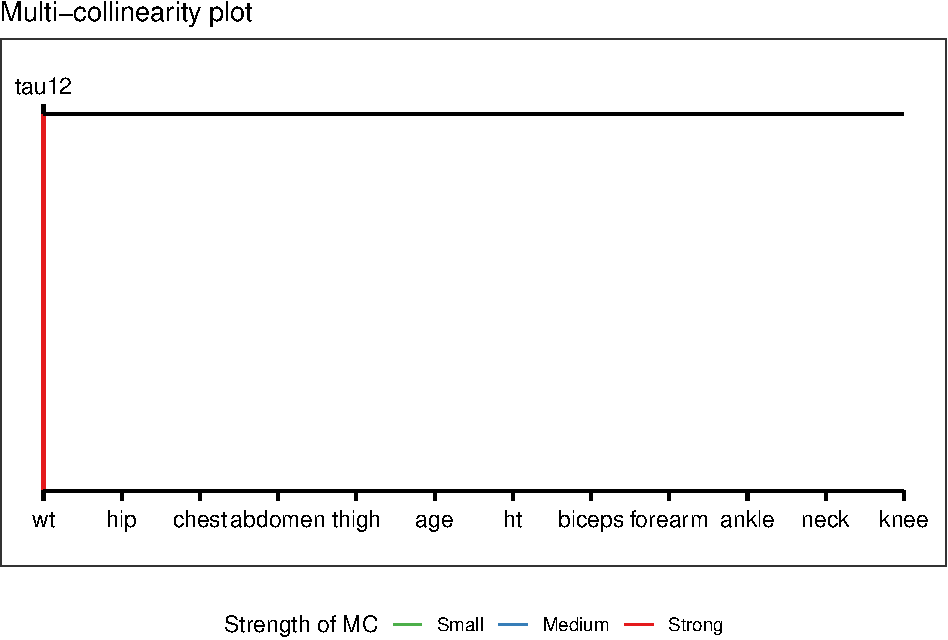
\includegraphics{BodyFat_files/figure-latex/unnamed-chunk-45-1.pdf}

Remove wt

\begin{Shaded}
\begin{Highlighting}[]
\NormalTok{X =}\StringTok{ }\KeywordTok{cbind}\NormalTok{(age,ht,neck,chest,abdomen,hip,thigh,knee,}
\NormalTok{         ankle,biceps,forearm)}
\NormalTok{mcvis_result =}\StringTok{ }\KeywordTok{mcvis}\NormalTok{(}\DataTypeTok{X =}\NormalTok{ X)}
\NormalTok{mcvis_result}
\end{Highlighting}
\end{Shaded}

\begin{verbatim}
##       age   ht neck chest abdomen hip thigh knee ankle biceps forearm
## tau11   0 0.01 0.01  0.08    0.75 0.1  0.02 0.02  0.01   0.01    0.01
\end{verbatim}

\begin{Shaded}
\begin{Highlighting}[]
\KeywordTok{plot}\NormalTok{(mcvis_result)}
\end{Highlighting}
\end{Shaded}

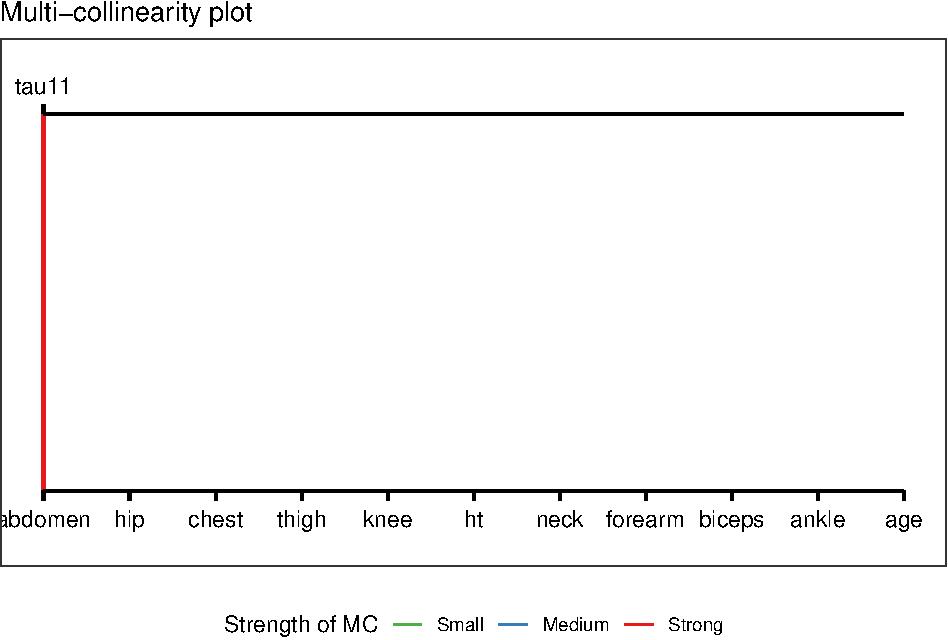
\includegraphics{BodyFat_files/figure-latex/unnamed-chunk-47-1.pdf}

Remove Abdomen

\begin{Shaded}
\begin{Highlighting}[]
\NormalTok{X =}\StringTok{ }\KeywordTok{cbind}\NormalTok{(age,ht,neck,chest,hip,thigh,knee,}
\NormalTok{         ankle,biceps,forearm)}
\NormalTok{mcvis_result =}\StringTok{ }\KeywordTok{mcvis}\NormalTok{(}\DataTypeTok{X =}\NormalTok{ X)}
\NormalTok{mcvis_result}
\end{Highlighting}
\end{Shaded}

\begin{verbatim}
##        age   ht neck chest hip thigh knee ankle biceps forearm
## tau10 0.01 0.02 0.01  0.05 0.4  0.49 0.01     0      0    0.01
\end{verbatim}

\begin{Shaded}
\begin{Highlighting}[]
\KeywordTok{plot}\NormalTok{(mcvis_result)}
\end{Highlighting}
\end{Shaded}

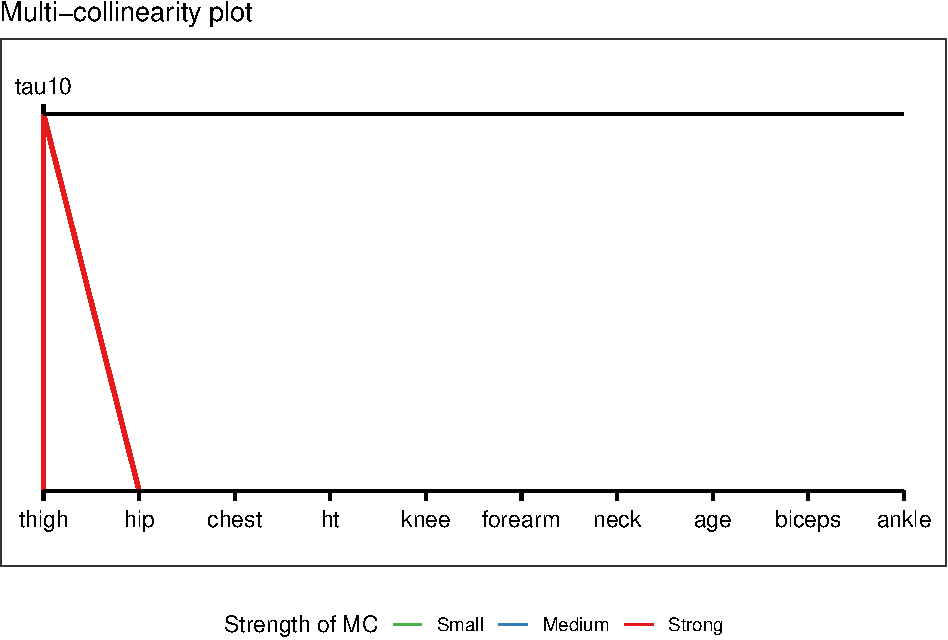
\includegraphics{BodyFat_files/figure-latex/unnamed-chunk-49-1.pdf}

Remove thigh

\begin{Shaded}
\begin{Highlighting}[]
\NormalTok{X =}\StringTok{ }\KeywordTok{cbind}\NormalTok{(age,ht,neck,chest,hip,knee,}
\NormalTok{         ankle,biceps,forearm)}
\NormalTok{mcvis_result =}\StringTok{ }\KeywordTok{mcvis}\NormalTok{(}\DataTypeTok{X =}\NormalTok{ X)}
\NormalTok{mcvis_result}
\end{Highlighting}
\end{Shaded}

\begin{verbatim}
##       age ht neck chest hip knee ankle biceps forearm
## tau9 0.01  0 0.01  0.12 0.7 0.06  0.01   0.01    0.09
\end{verbatim}

\begin{Shaded}
\begin{Highlighting}[]
\KeywordTok{plot}\NormalTok{(mcvis_result)}
\end{Highlighting}
\end{Shaded}

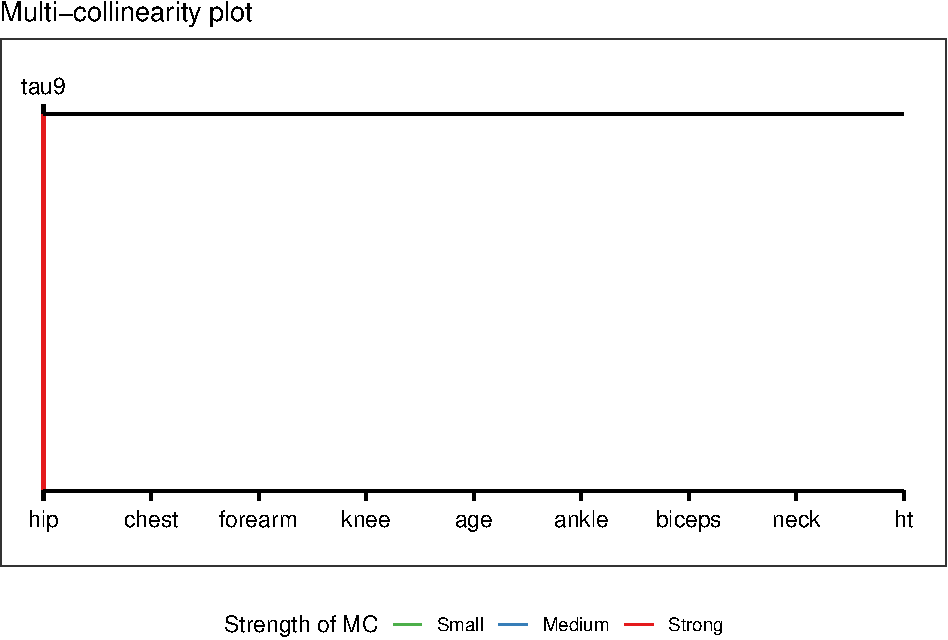
\includegraphics{BodyFat_files/figure-latex/unnamed-chunk-51-1.pdf}

\end{document}
